\section{Justificativa de reentrega}

Estou enviando esse trabalho com o objetivo de apresentar o documento (em PDF e TEX) e um novo código fonte desenvolvido para o trabalho após entender sobre a correta aplicação de um método eficaz para o encontro dos caminhos disjuntos.

Pelos fatos citados acima e por ter enviado erroneamente um trabalho de outra matéria por desatenção na primeira entrega, refiz esse trabalho com o objetivo de apresenta-ló mais bem redigido, alcançando um melhor desempenho, desde formato de apresentação, formatação do documento, organização dos conteúdos e qualidade do código.

Agradeço pela compreensão e abertura para essa entrega da atividade repositiva.

\section{Contextualização}

Um caminho simples em um grafo direcionado é um caminho sem vértices repetidos. Mais precisamente, um caminho é uma sequência (v0, a1, v1, a2, v2, . . . , ak, vk) com k >= 1 em que v0, v1, v2, . . . , vk são distintos dois a dois. Em grafos simples, pode-se representar um caminho apenas pela sequência de vértices (uma vez que só pode existir uma única aresta entre cada par de vértices). No grafo ilustrado na Fig. 1 as sequências (A, B, E, F ) e (A, D, C, F ) são exemplos de caminhos simples. Além disso, esses dois caminhos são disjuntos em arestas pois não possuem nenhuma aresta em comum.

O problema de se determinar o número máximo de caminhos disjuntos em arestas existentes em um grafo apresenta várias aplicações. Neste trabalho você deverá implementar um método de resolução deste problema que receba um grafo e um par de vértices (isto é, origem e destino) exiba ao final a quantidade de caminhos disjuntos em arestas entre os dois vértices dados, além de listar cada um dos caminhos encontrados.
\\
\\
Numa lista de tarefas, devemos implementar no algoritmo as seguintes regras:

\begin{itemize}
  \item método de resolução deste problema que receba um grafo e um par de vértices (isto é, origem e destino)
  \item exiba ao final a quantidade de caminhos disjuntos em arestas entre os dois vértices
  \item listar cada um dos caminhos encontrados.
\end{itemize}


% descrevendo detalhes da implementação, dos experimentos e resultados obtidos.

%xiba ao final a quantidade de caminhos disjuntos em arestas entre os dois vértices dados, além de listar cada um dos caminhos encontrados.

\subsection{Lógica}

Nesse trabalho devemos encontrar o número máximo de caminhos disjuntos em arestas existentes em um grafo. O código deve apresentar a quantidade de caminhos disjuntos em arestas entre os dois vértices dados e listar cada um dos caminhos encontrados.

Temos algumas formas de fazer essa busca, entretanto, algumas delas não são buscas consideradas ótimas, como é o caso do BFS com exclusão de arestas.

Como no caso do exemplo abaixo que chegamos do vértice D saindo do A e encontramos apenas um caminho "ótimo", visto o algoritmo.
\begin{center}
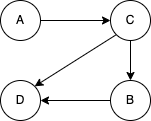
\includegraphics[width=5cm, height=4cm]{figuras/01.png}
\end{center}

\subsection{Lógica Ótima}
Pensando que devemos ter uma lógica ótima, devemos ter um algoritmo que não delete as arestas e que encontre e mostre o número máximo e atenda todas as expectativas.

Podemos então utilizar como base o algoritmo de fluxo em rede, como no caso do de Ford Fullkerson para realizar todas as tarefas e encontrar os caminhos disjuntos, mostrando-os e contabilizando-os.

\section{Definições}

\subsection{Par de caminhos disjuntos}
Um par de caminhos (por meio de vértices) em um grafo é considerado disjunto se e somente se não possuírem arestas em comum, ou seja, se nenhuma aresta do grafo é utiliza por ambos os caminhos.

Exemplo: No grafo definido abaixo, os caminhos (1,2,4) e (1,3,4) são disjuntos.  Já os caminhos (1,2,3,4) e (1,3,4) não são disjuntos.

\begin{center}
  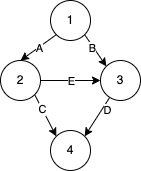
\includegraphics[ height=4cm]{figuras/02.png}
\end{center}


\subsection{Rede de Fluxo}
Uma rede de fluxo é um grafo direcionado G = (N, A), com N como conjunto de nós e A o conjunto de arestas, com as seguintes propriedades:
\\
\\
- Para cada aresta $a \in A$ há um número não negativo $C_{a}$, que indica a capacidade da mesma (ou seja, a quantidade máxima de fluxo que cada uma é capaz de carregar).\\
- Existe um único nó que será identificado como fonte (source), a ser denotado por s;\\
- Existe um único nó que será identificado como terminal (ou sumidouro) t, tal que $t \in N$;\\
- Não há nenhuma aresta direcionada para a fonte s, apenas arestas que saem dela e são direcionadas para outros nós.\\
- Não há nenhuma aresta que saia do terminal t, apenas arestas direcionadas a ele.


\section{Escolha do algoritmo}

\\

Para encontrar o número máximo de caminhos disjuntos podemos utilizar alguns algoritmos, entretanto como citado acima um deles é considerado ótimo. Ao escolher um BFS ou DFS como algoritmo alguns casos terão sucesso, porém em outros teremos erros que consideram caminhos disjuntos falsos, ou até mesmo a falta deles.
\\

Utilizei como base o algoritmo de Ford-Fulkerson para a solução do problema, utilizando como fluxo máximo em cada aresta começando em zero respeitando as seguintes propriedades:
\\
\\
Restrições de capacidade: Para cada $a \in A$, temos que $0 <= f(a) <= c_{a} $
\\
Restrições de conservação: Para cada nó $n \in N$ diferente de $s$ e $t$, temos que o fluxo total que entra em determinado nó é igual ao fluxo total que sai de tal nó.

\subsection{O algoritmo de Ford-Fulkerson}
Iniciamos supondo que o fluxo inicial em todas as arestas é nulo, e com isso iremos aumentar acrescentando fluxo na fonte com algumas regras.

A ideia principal do algoritmo gira em torno de duas principais operações:
\begin{itemize}
  \item Quando uma aresta tem menos fluxo do que permite a sua capacidade (incluindo o fluxo nulo), podemos "empurrar"  fluxo em sua direção.
\item Quando uma aresta tem uma quantidade positiva de fluxo, menor ou igual à sua capacidade, podemos fazer com que esse fluxo retroceda, "empurrando-o para trás"
\end{itemize}
\newpage
Para tais operações do algoritmo, devemos utilizar um grafo auxiliar, que segundo as questões já definidas chamaremos de \textbf{Grafo Residual ({$G_{R}$})} seguindo também algumas regras:


\begin{itemize}
  \item O conjunto de nós $G_{R}$ é o mesmo de $G$
  \item Ao percorrer as arestas em $G$, vamos criando as arestas de $G_{R}$ da seguinte maneira:
  \\\\
   - Para cada aresta $a = (n_{i},n_{j})$ de $G$ - (sai do nó $n_{i}$ e entra no nó $n_{j}$) - que possui fluxo $f(a) < c_{a}$, adicionamos uma aresta $a_{R} = (n_{i},n_{j})$ com capacidade $c_{aR}$ = $c_{a} - f(a) e f(a_{r})$ = 0. Deste modo, estamos definindo a possibilidade de "empurrar para frente" a quantidade de fluxo que a aresta $a$ conseguiria carregar a mais.
   \\\\
   - Para cada aresta $a = (n_{i},n_{j})$ de $G$ tal que $f(a) > 0$, ou seja, cada aresta que já esteja carregando alguma quantidade positiva de fluxo, existe a possibilidade de empurrar este fluxo para trás, se assim desejarmos. Desta forma, adicionamos uma aresta $a{'}_{R} = (n_{i},n_{j})$  em $G_{R}$ com direção inversa a $a$ e a capacidade $c_{a{'}_{R}} = f(a)$. Assim como no passo anterior, o fluxo de $a{'}_{R}$ no grafo residual é nulo.
\end{itemize}
\newpage

